\documentclass[11pt]{jsarticle}

\usepackage{amsmath,amsthm,amssymb}
\usepackage[dvipdfmx]{graphicx}
\usepackage{bm}
%
\usepackage{multirow}
\usepackage{wrapfig}
%
\pagestyle{empty}
%% 高さの設定
\setlength{\textheight}{\paperheight}   % ひとまず紙面を本文領域に
\setlength{\topmargin}{-5.4truemm}      % 上の余白を20mm(=1inch-5.4mm)に
\addtolength{\topmargin}{-\headheight}  % 
\addtolength{\topmargin}{-\headsep}     % ヘッダの分だけ本文領域を移動させる
\addtolength{\textheight}{-40truemm}    % 下の余白も20mmに%% 幅の設定
\setlength{\textwidth}{\paperwidth}     % ひとまず紙面を本文領域に
\setlength{\oddsidemargin}{-5.4truemm}  % 左の余白を20mm(=1inch-5.4mm)に
\setlength{\evensidemargin}{-5.4truemm} % 
\addtolength{\textwidth}{-40truemm}     % 右の余白も20mmに

%
\abovecaptionskip=-1pt
%\belowcaptionskip=-1pt
%
\renewcommand{\baselinestretch}{0.92} % 全体の行間調整
\renewcommand{\figurename}{Fig.}
\renewcommand{\tablename}{Tab.}
%
\makeatletter 
\def\section{\@startsection {section}{1}{\z@}{1.5 ex plus 2ex minus -.2ex}{0.5 ex plus .2ex}{\large\bf}}
\def\subsection{\@startsection{subsection}{2}{\z@}{0.2\Cvs \@plus.5\Cdp \@minus.2\Cdp}{0.1\Cvs \@plus.3\Cdp}{\reset@font\normalsize\bfseries}}
\makeatother 
%

\begin{document}

%%%%%%
% はじめに
%%%%%%
\begin{center}
{\Large \textgt{1. MD シミュレーションによるネットワークポリマーのゴム弾性}}
\end{center}

\begin{flushright}
東亞合成 佐々木裕

Tel: 052-611-9923, e-mail: hiroshi\_sasaki$@$mail.toagosei.co.jp
\end{flushright}

\vspace{0.5\baselineskip}
\section{はじめに}

%近年、ソフトマターの階層的な構造設計の考え方が深化し、力学特性に優れたネットワークポリマーの材料設計にも応用されている。
%例えば、旧知の材料であるゴムの機能性の発現機構についても、フィラーとの相互作用~\cite{Igarashi2013}という観点から精力的に検討されている。
%また、脆い材料として知られているゲルも、これまでにない高強度なものが発見されてきている~\cite{Gong2010}。
%これらのネットワークポリマーの材料設計においては、フィラー同士の相互作用のような比較的大きなスケールの構造から、
%フィラーとエラストマー界面近傍での拘束領域のような中間的なスケール、さらには、
%ネットワーク構造の均一性のようなミクロなスケールに至るマルチスケールの事象が、階層的に組み合わさってマクロな特性に大きな影響を与えることが知られている~\cite{Deng2010}。

%軽量化した新規複合材料の開発において高分子材料の高靭性化は重要な問題であり、その発現機構の解明を含めた検討が期待されている。
従来の金属材料からの大幅な軽量化を目指した新規複合材料の開発において、高分子材料は重要な役割を占めている。
その際の最も重要な問題として信頼性の不足が指摘され、耐久性向上(高靭性化)が望まれている。
材料の耐久性とは、「破壊」や「疲労」への耐性と捉えることができ、「Griffith 理論」での亀裂進展に伴うエネルギー開放率 $G_c$、さらには、$J$ 積分により非線形領域へ拡張された $J_c$ が破壊にたいする靭性の指標となると考えられている。
ただし、破断時の変形がけた違いに大きいゴム材料への適応には注意が必要であり、粘弾性効果の影響が少ない高温、低速での破壊においては、Lake \& Thomas の指摘~\cite{Lake1967}するように、亀裂先端近傍での架橋点間のストランドの破断というモデルが成立するようであるが、実際にゴム材料を使用するような条件下においては、ゴムの破壊靭性値は遥かに大きなものとなっている。

Andrews は、応力 - ひずみ関係におけるヒステリシスに着目し、ヒステリシスロスの存在により亀裂先端での荷重場と除荷場との間での亀裂進展に伴うエネルギー開放量が減少し、結果として亀裂の進展が抑制されるモデルを提案している~\cite{Andrews1977}。
確かに、旧知の材料であるゴムにおけるフィラーの効果~\cite{Igarashi2013}や、強靭なゲルとして知られているダブルネットワーク・ゲルにおける犠牲結合モデル~\cite{Gong2010}においては大きなヒステリシスが存在する。
それらの高靭性メカニズムはこの考え方に合致し、比較的大きいメゾスケール領域での亀裂進展に伴うエネルギー散逸と捉えることができる。

このような強靭化モデルは、このスケールでしか発現しないのであろうか。
我々は、ネットワークの分子鎖描像のようなミクロな領域においても粘弾性緩和でのエネルギー散逸を設計することでエラストマー材料の破壊耐性を向上し、しなやかな強さを付与できる可能性が残されているのではないかと考えている。

ゴム弾性の古典的なモデルは、ネットワークを構成するストランドをガウス鎖とし、その結節点のミクロな変形がマクロな変形と相似でアフィン変形するとした「ネオ・フッキアンモデル」が知られている。
ミクロな分子鎖描像の有効な一手法である分子動力学(MD)シミュレーションによる「KG 鎖」と呼ばれるビーズ・スプリングモデル~\cite{Kremer1990} をストランドとする規則構造を有するネットワークを用いて、Everaers らは、各種のゴム弾性理論との高い整合性を報告している~\cite{Everaers1999}。
この古典的なモデルからの発展形として、結節点の揺らぎに注目しミクロな変形がマクロと異なるとした「ファントムネットワークモデル~\cite{Flory1976}」が提案されており、メルト状態と同一な鎖長の分布関数を有するランダムネットワークにおいて「ファントムネットワーク」としてのふるまいを示すとされている。
我々は、この結節点のゆらぎ由来の散逸が、ミクロなスケールでの粘弾性的なエネルギー散逸モデルとなりうるのではないかと考えている。

本報告では、規則構造ネットワークのユニットセル間における規則性をランダムへと変えることで、「ファントムネットワークモデル」を再現できるシミュレーション系の構築を目指し、平衡構造での鎖の挙動、及び、大変形時の挙動に注目した検討結果について報告する。

\section{シミュレーション}
%\vspace{-2mm}

\subsection{ネットワークモデルの作成}

任意の分岐数$f$($f=3\sim6$)の結節点からなる規則構造を有するネットワークに対して、トポロジーモデルの「代数的連結性」を指標として以下のアルゴリズムでランダムな結合性を導入した。
\vspace{-2mm}
\begin{enumerate}
\item
実空間で"8-Strand Unit Cell"の周期境界での連なり(2x2x2=8 Cells の例)の初期構造(Fig. \ref{fig:cells})。
\item
初期構造に対応したトポロジーモデルを用いてノードごとのエッジ数(分岐数)に変換(Fig. \ref{fig:topo})。
\item
トポロジーモデルにて、ネットワークの結びつきの強さを表す代数的連結性を指標として連結性を維持しながらストランド交換し、結節点の結合性にランダム性を導入(Fig. \ref{fig:exc})。
\item
そのトポロジーモデルに対応するように、実空間の初期構造からストランドを除去。
\end{enumerate}

\vspace{1mm}
\begin{figure}[hb]
\begin{minipage}{0.33\hsize}
	\begin{center}
	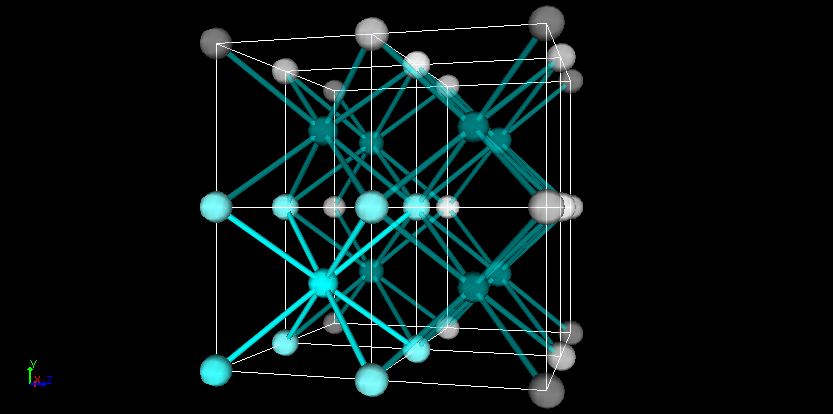
\includegraphics[width=50mm]{./fig/8_per.png}
	\caption{$2^3$ of 8-Strand Unit Cells}
	\label{fig:cells}
	\end{center}
\end{minipage}
\begin{minipage}{0.33\hsize}
	\begin{center}
	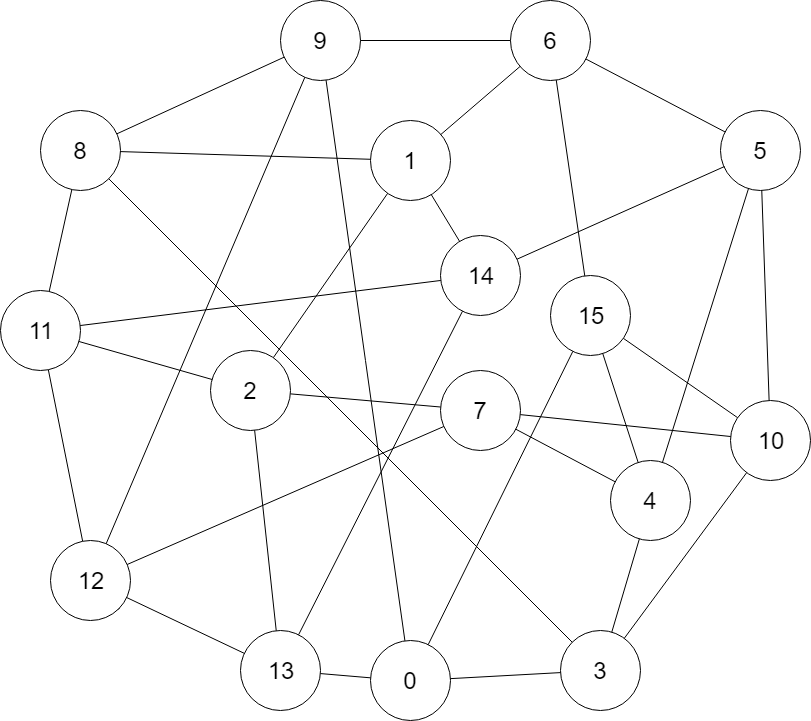
\includegraphics[width=30mm]{./fig/Network.png}
	\caption{Topological NW Model}
	\label{fig:topo}
	\end{center}
\end{minipage}
\begin{minipage}{0.33\hsize}
	\begin{center}
	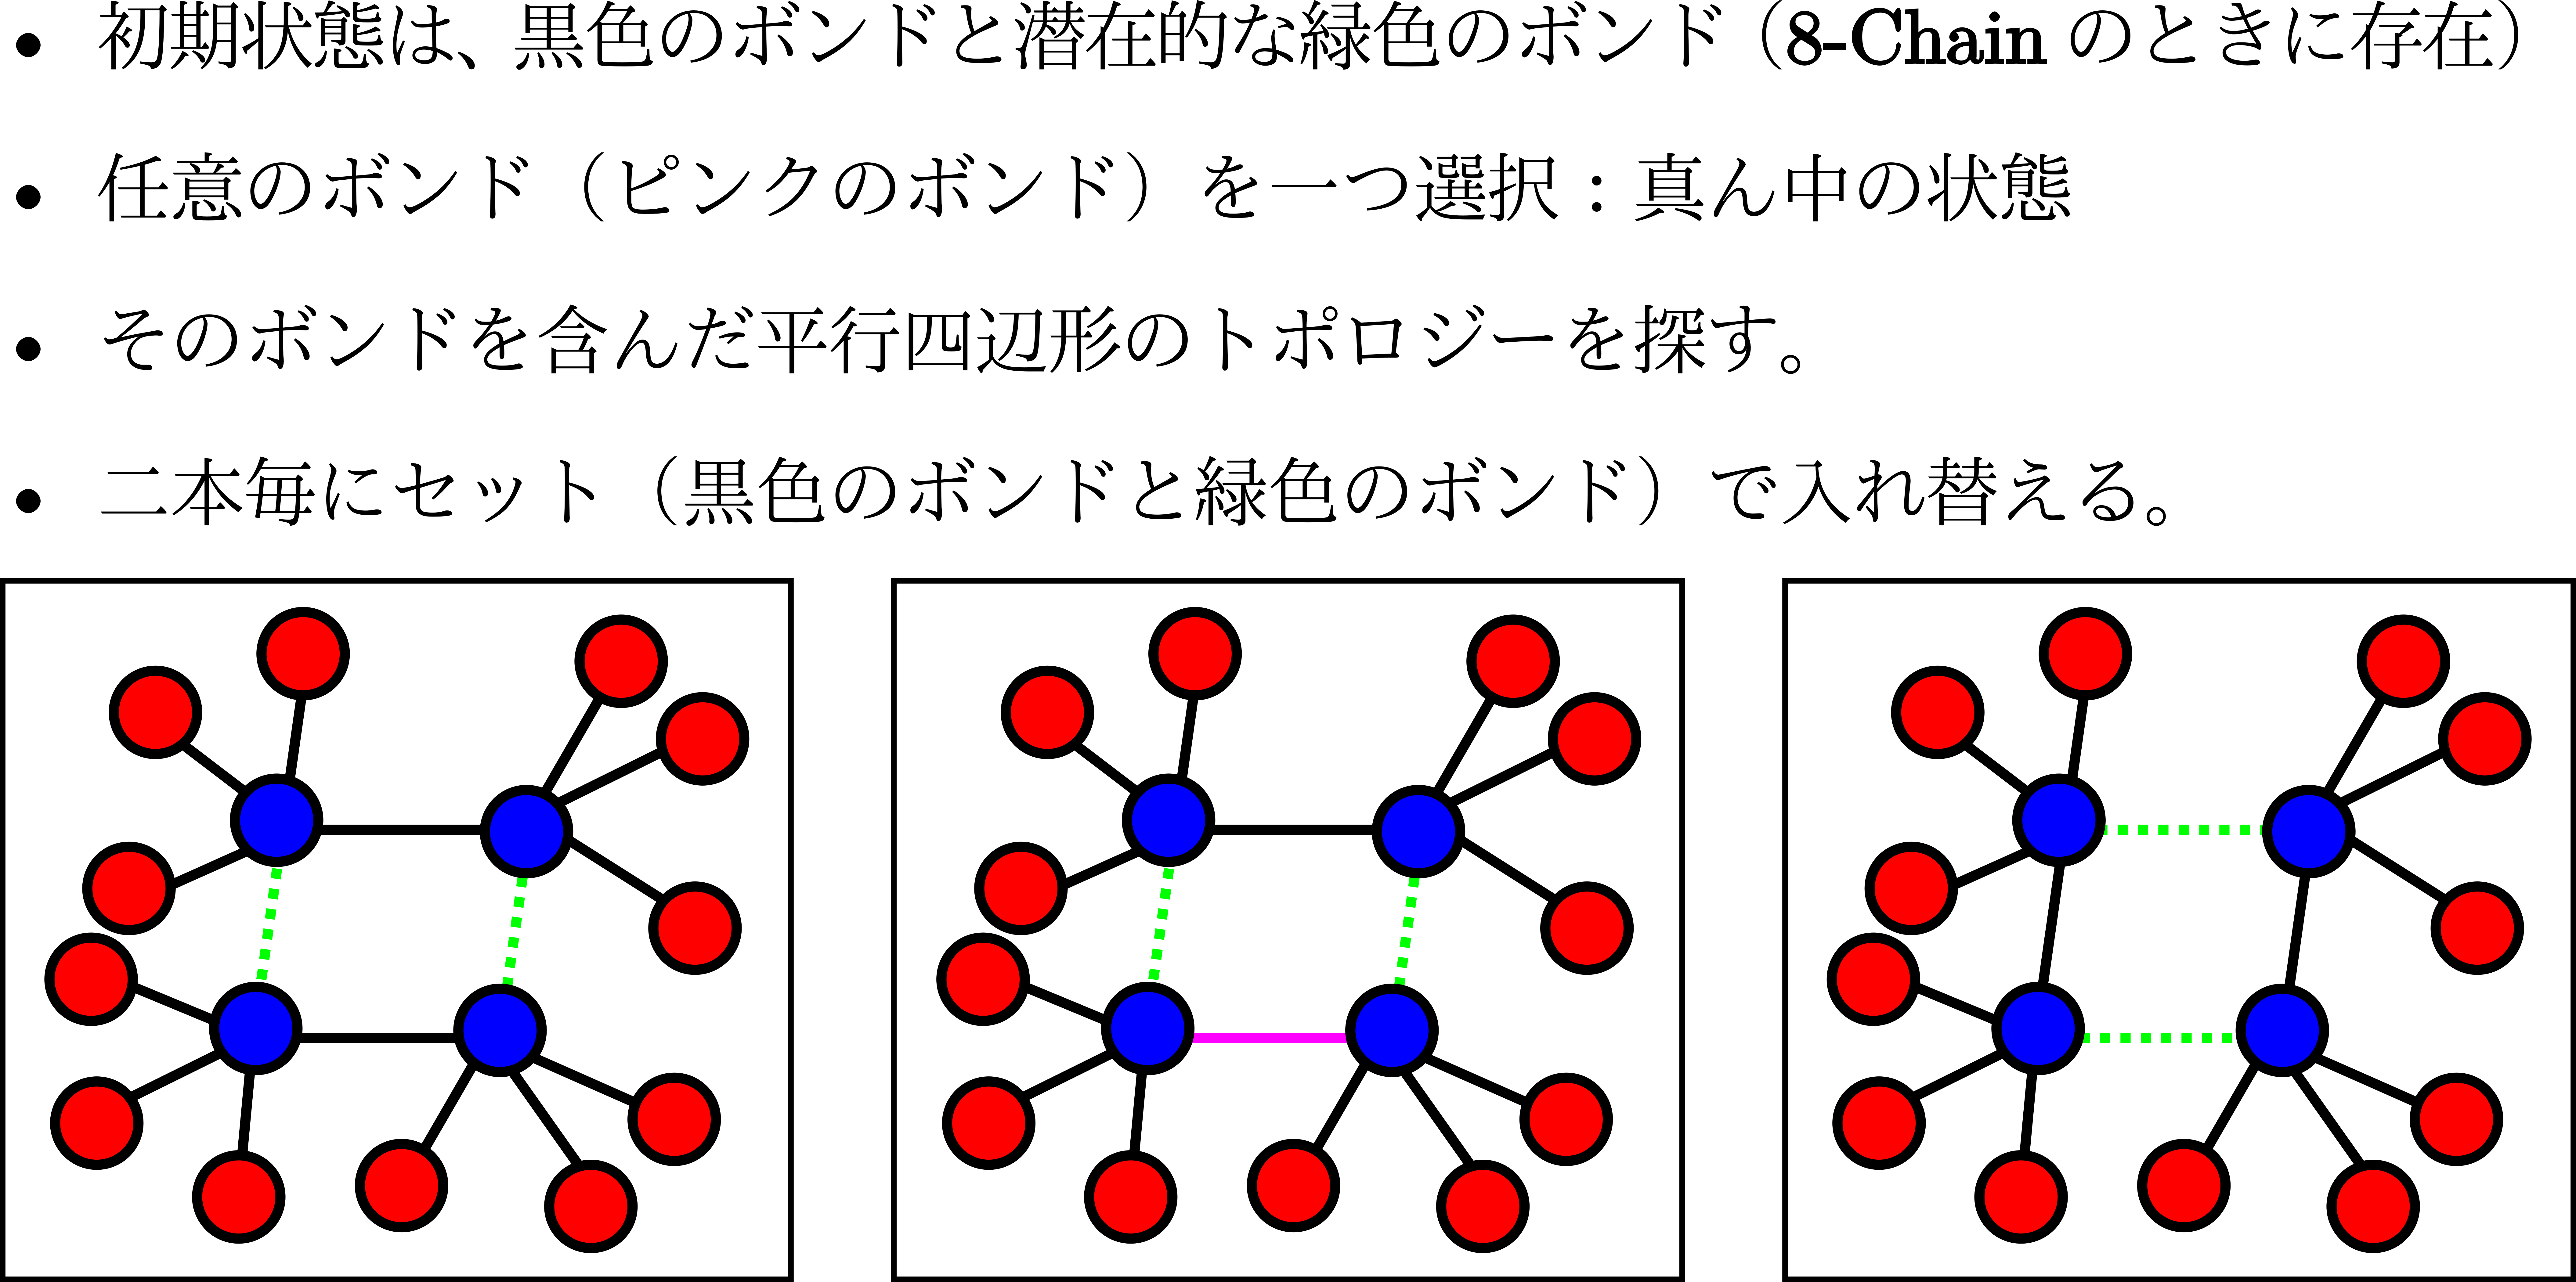
\includegraphics[width=50mm]{./fig/ボンド交換.png}
	\caption{Strand Exchange Procedure}
	\label{fig:exc}
	\end{center}
\end{minipage}
\end{figure}
\vspace{-3mm}


\subsection{MD シミュレーション}

上記にて生成したランダムな結合性を有するネットワーク(ストランドの末端間距離をメルトの特性比 $C_N = 1$ に設定)を、
%その平衡状態および一軸伸長時の振る舞いについて、
OCTA 上の COGNAC シミュレーターにより MD シミュレーションを行った。

%非結合ポテンシャルとして各ビーズ間に斥力相互作用($r_c = 2^{(1/6)}\sigma$)である LJ ポテンシャル $U_{LJ}(r_{ij})$、ボンドポテンシャルには、$U_{FENE}(r)$ と斥力 LJを合わせた FENE-LJ ポテンシャルを用いた。
%ファントム鎖は非結合ポテンシャルを省略し、ボンドポテンシャルに FENE-LJ、あるいは、ハーモニックポテンシャル($k=30$)とした。

%\vspace{-2mm}
%\begin{align*}
%\tiny
%&U_{LJ}( r_{ij} ) =
%\begin{cases}
%4\epsilon_{LJ} \left[ \left( \dfrac{ \sigma }{ r_{ij} } \right)^{12} - \left( \dfrac{ \sigma }{ r_{ij} } \right)^{6} \right] \; & r_{ij}< r_c \\[8pt]
%0 \; & r_{ij} \geq r_c
%\end{cases} \\[10pt]
%&U_{FENE}( r ) = 
%\begin{cases}
%-\dfrac{1}{2} k R_0^2 \ln \left[ 1 - \left( \dfrac{ r }{ R_0 } \right)^{2} \right]  \; & r < R_0 \\[8pt]
%\infty \; & r \geq R_0
%\end{cases} \\
%&\; where \; R_0 = 1.5 \sigma, k = 30
%\end{align*}
%
%\vspace{-5mm}
%\begin{figure}[htb]
% \centering
%	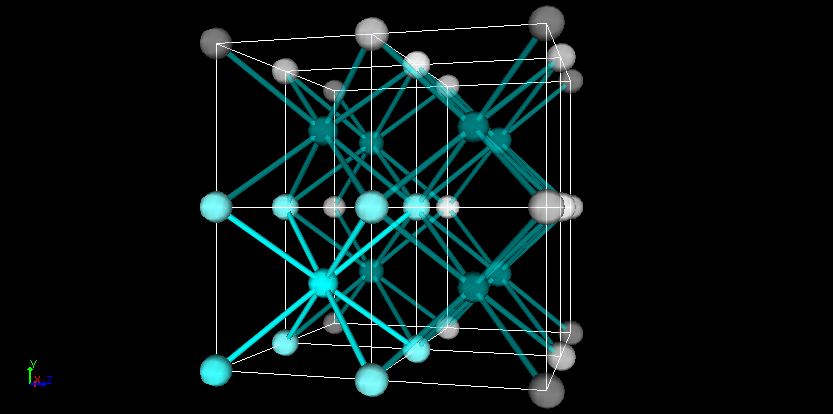
\includegraphics[width=50mm]{./fig/8_per.png}
%	\caption{2x2x2 Cells of 8 strands}
%	\label{fig:cells}
%\end{figure}
%\vspace{-5mm}




\section{結果と考察}
%\vspace{-2mm}
セグメント間の非結合ポテンシャルを省略した「す拔け鎖」をストランド(セグメント数 $N = 50$ )、ストランドの末端間距離をメルトと同一に設定した四分岐モデル(5x5x5 Cells)の結果についてまとめた。

\subsection{トポロジーモデルの結節点のランダム性の評価}

上記のモデルにおいて、結節点の繋ぎ変えを 100,000 回サンプリングした場合のネットワークの結びつきの強さを表す指標である代数的連結性の分布関数を Fig. \ref{fig:alg} に示した。
この分布の最頻値近傍のトポロジーモデルを実空間でのシミュレーションモデルの初期構造とした。

\subsection{ストランドの末端間距離 $\langle \bm{R} \rangle$ の分布関数}

初期緩和後のストランドの末端間距離の分布関数を Fig. \ref{fig:e2e} に示した。
初期設定と比較して末端間距離が伸び(特性比 $C_N \simeq 1.36$)、ファントムネットワークモデルで予想される振る舞いとほぼ合致した。

%\begin{align*}
%R=
%\end{align*}


\vspace{-1mm}
\begin{figure}[hb]
\begin{minipage}{0.5\hsize}
	\begin{center}
	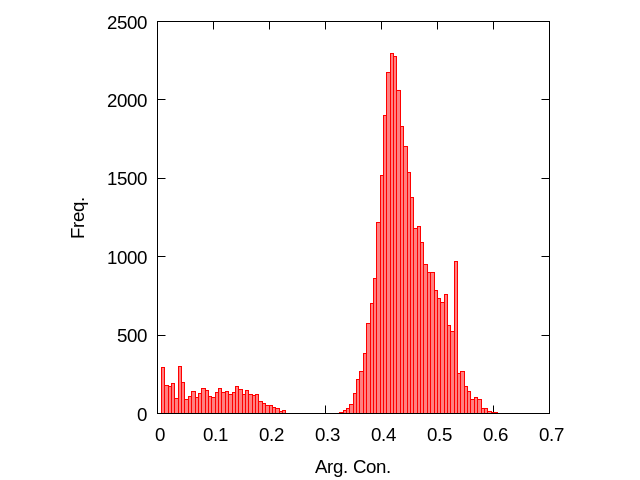
\includegraphics[width=65mm]{./fig/Histgram.png}
	\caption{Algebraic Connectivity Histogram for 4-Chain Model with 5x5x5 Cells with 100,000 times Samplings}
	\label{fig:alg}
	\end{center}
\end{minipage}
\begin{minipage}{0.5\hsize}
	\begin{center}
	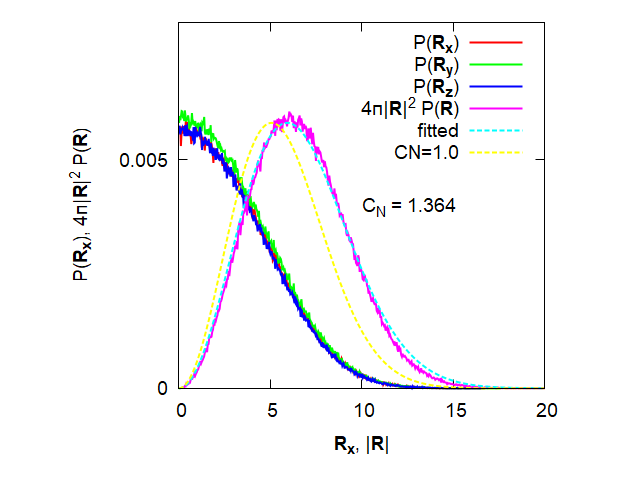
\includegraphics[width=65mm]{./fig/Strand_histgram.png}
	\caption{End to End Distribution of Strands for 4-Chain Model with 5x5x5 Cells after Equilibration }
	\label{fig:e2e}
	\end{center}
\end{minipage}
\end{figure}

\vspace{-3mm}

\bibliographystyle{achemso}
\bibliography{D:/Dropbox/Tex/Bibliography/library.bib}

\end{document}